\chapter{Computational Fluid Dynamics}

\section{Tools}

\subsection{XFOIL}

XFOIL is a program for the analysis of subsonic isolated airfoils developed at the Massachusetts Institute of Technology.

\subsection{VSPAERO}

VSPAERO is a combined vortex lattice method (VLM) and panel method solver integrated with OpenVSP, a parametric aircraft geometry tool developed at NASA Ames Research Center. VSPAERO can be used to compute aircraft aerodynamic characteristics within linear range of the lift. \cite{Litherland2015-1} OpenVSP allows users to fast create an aircraft 3D model by defining geometric parameters.

\subsection{OpenFOAM}

OpenFOAM is an open source software for computational fluid dynamics (CFD) originally created at Imperial College London. OpenFOAM contains various solvers intended to simulate different physical phenomena.

\section{Workflow}

\subsection{XFOIL}

Follow this steps to obtain airfoil characteristics. Notice that XFOIL commands are case sensitive. \cite{DrelaYoungren2001}

\begin{enumerate}
  \item Open terminal and execute \texttt{xfoil} program. \\
  XFOIL command promt should start.
  \item Read buffer airfoil from coordinate file with \texttt{LOAD} command e.g \texttt{LOAD~2412.dat}, or set NACA 4 or 5 digit airfoil with NACA command e.g. \texttt{NACA~2412}. \\
  Coordinate file is a simple text file which contains list of the 2D airfoil coordinate points starting at the trailing edge, progressing to the leading edge along the upper surface, and returning to the trailing edge along the lower surface.
  \item Set number of panel nodes to at least 160 with \texttt{PPAR} command if necessary.
  \item Enter operation mode with \texttt{OPER} command. \texttt{OPERi} indicates inviscid mode.
  \item Enter viscous mode with \texttt{Visc} command. \\
  Enter Reynolds number for typical flight conditions. \texttt{OPERv} should appear.
  \item Set Mach number for typical flight conditions with \texttt{Mach} command.
  \item Specify output files with \texttt{Pacc} command.
  \item Specify the angle of attack range and run computations with \texttt{Aseq} command.
\end{enumerate}

\subsection{VSPAERO}

\begin{figure}
  \centering
  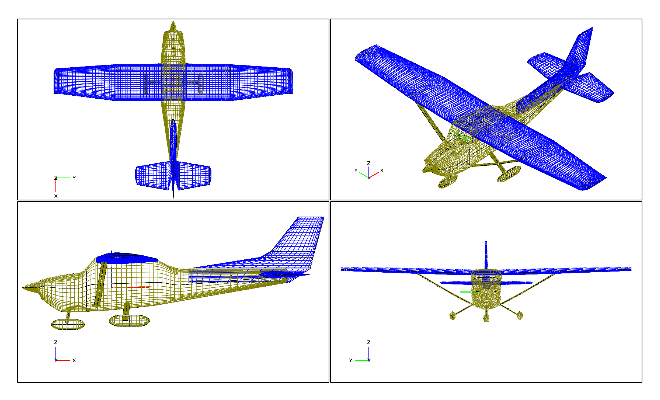
\includegraphics[width=120mm]{images/vspaero_01.eps}
  \caption{OpenVSP aircraft model}
\end{figure}

An appropriately define aircraft 3D model is needed to analyze. \cite{Litherland2015-2} Based on this model degenerated geometry file is generated for the vortex lattice method and surface triangulation file for the panel method.

\begin{figure}
  \centering
  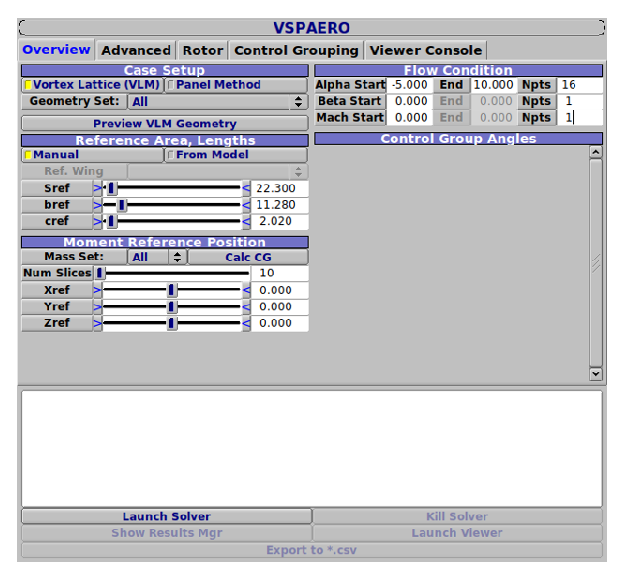
\includegraphics[width=100mm]{images/vspaero_02.eps}
  \caption{VSPAERO computations setup GUI}
\end{figure}

VSPAERO can be run from within Analysis menu of the OpenVSP. Some additional setup should be done to start computations. Vortex lattice method or panel method solver should be chosen. Reference area, lengths and moment reference position should be specified to get correct results. Angle of attack range should be specified for the linear range of the lift. Critical angle of attack can be calculated using formula (\ref{eq-aero-alpha-critical}). Mach number should be set to typical flight conditions.

VSPAERO Viewer and Results Manager can be used to visualize results. Computed aerodynamic characteristics are saved as plain text files, which are both easy to understand by a human and easy to read by a computer program.

\begin{figure}
  \centering
  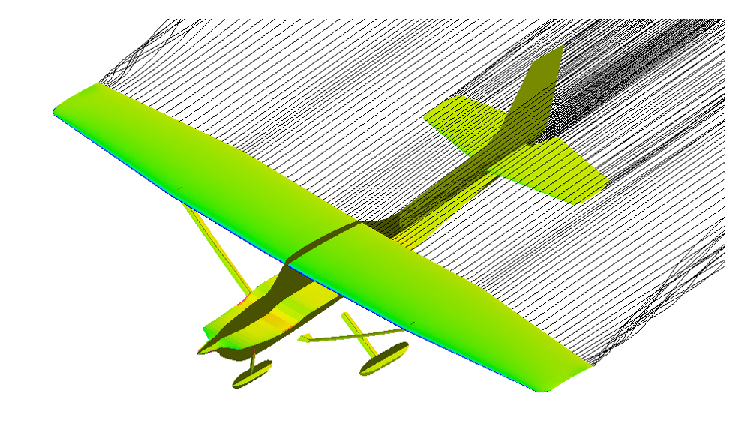
\includegraphics[width=120mm]{images/vspaero_03.eps}
  \caption{Wakes and pressure coefficient change distribution}
\end{figure}

\subsection{OpenFOAM}

\subsubsection{Solver}

OpenFOAM \texttt{simpleFoam} is a steady-state solver for incompressible, turbulent flow using SIMPLE (Semi-Implicit Method for Pressure Linked Equations) algorithm, which can be used to compute aircraft aerodynamic characteristics for the full range of angle of attack. \cite{Greenshields2018, MoukalledManganiDarwish2016, VersteegMalalasekera2007}

SST k-$\omega$ Reynolds-Averaged Navier-Stokes (RANS) turbulence model is used.

\subsubsection{Mesh -- Control Volume}

OpenFOAM \texttt{blockMesh} utility is used to create control volume mesh defined in \texttt{system/blockMeshDict} dictionary file as a mesh composed of hexahedral blocks.

The simplest case is when the control volume is defined by exactly one rectangular prisms.

\begin{figure}[h!]
  \centering
  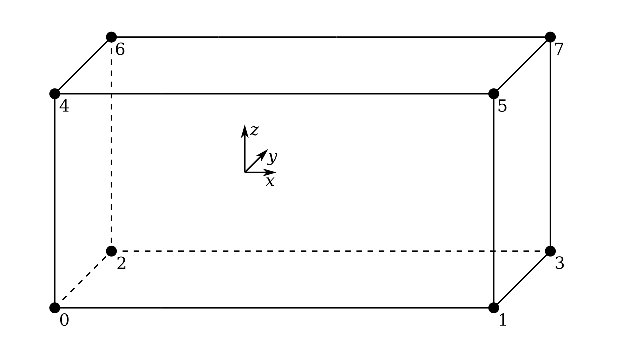
\includegraphics[width=100mm]{images/openfoam_control_volume_1_1.eps}
  \caption{Basic control volume scheme}
\end{figure}

\begin{figure}[h!]
  \centering
  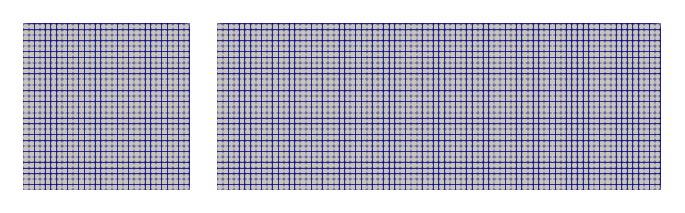
\includegraphics[width=110mm]{images/openfoam_control_volume_1_1_para.eps}
  \caption{Basic control volume mesh}
\end{figure}

Dictionary file is listed below:
\begin{codelistdict}
  \lstinputlisting{code/blockMeshDict_1}
\end{codelistdict}

\subsubsection{Mesh -- Simple Grading}

\begin{figure}[h!]
  \centering
  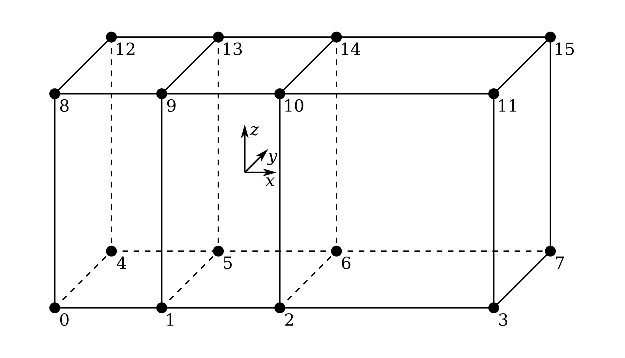
\includegraphics[width=100mm]{images/openfoam_control_volume_2_1.eps}
  \caption{Graded control volume scheme}
\end{figure}

\begin{figure}[h!]
  \centering
  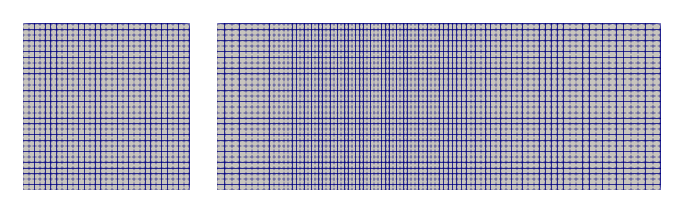
\includegraphics[width=110mm]{images/openfoam_control_volume_2_1_para.eps}
  \caption{Graded control volume mesh}
\end{figure}

Grading is used to increase mesh resolution in regions of interest. Due to create graded control volume mesh it has to be divided into subdomains. Scheme of control volume mesh one dimension grading is presented below.

Dictionary file is listed below:
\begin{codelistdict}
  \lstinputlisting{code/blockMeshDict_2}
\end{codelistdict}

\subsubsection{Mesh -- Complex Grading}

\begin{figure} [h!]
  \centering
  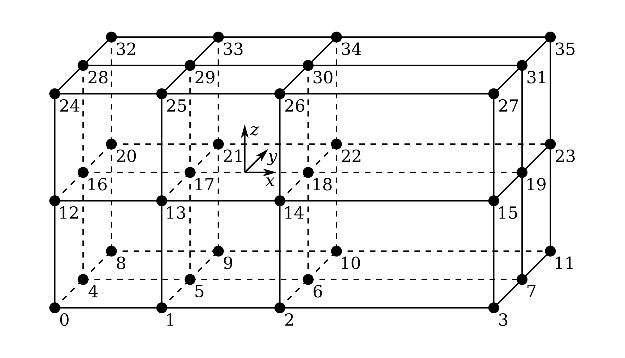
\includegraphics[width=100mm]{images/openfoam_control_volume_3_1.eps}
  \caption{Complex graded control volume scheme}
  \label{fig-cfd-mesh-complex-grading}
\end{figure}

\begin{figure} [h!]
  \centering
  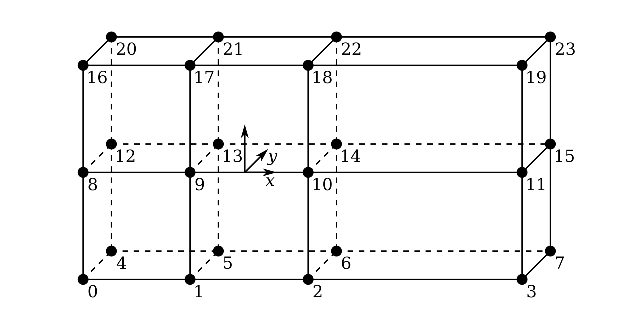
\includegraphics[width=100mm]{images/openfoam_control_volume_3_2.eps}
  \caption{Symmetric control volume scheme}
\end{figure}

Scheme of complex control volume mesh grading is presented on figure \ref{fig-cfd-mesh-complex-grading}.

For symmetric cases only half of the geometry can be considered to reduce computation time.

Dictionary file is listed below:
\begin{codelistdict}
  \lstinputlisting{code/blockMeshDict_3}
\end{codelistdict}

\subsubsection{Mesh -- Aircraft Geometry Model}

OpenVSP can be used to create aircraft 3D model and export it to STL. OpenFOAM \texttt{snappyHexMesh} utility is used to combine control volume mesh with aircraft geometry model. Volume near aircraft geometry can be refined due to achieve better results. Meshing parameters are specified in \texttt{system/snappyHexMeshDict} file.

\begin{figure}[h!]
  \centering
  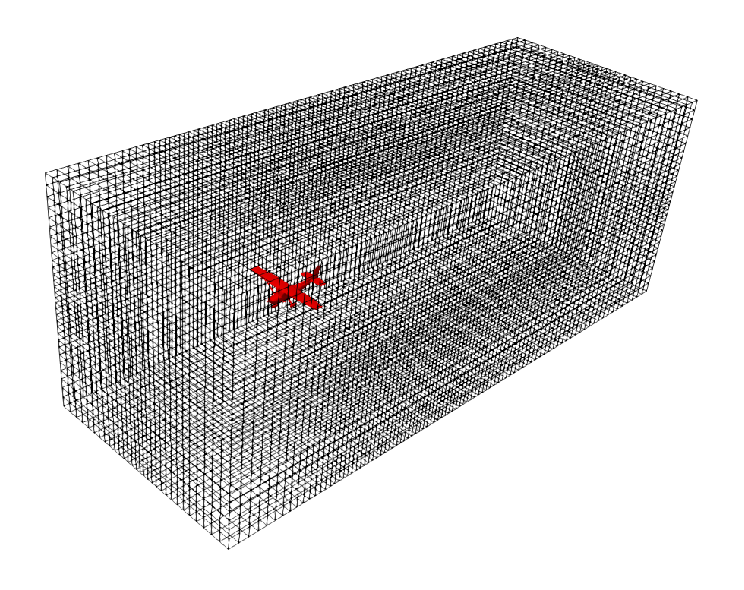
\includegraphics[width=120mm]{images/openfoam_mesh.eps}
  \caption{OpenFOAM complete mesh}
\end{figure}

\subsubsection{Initial and Boundary Conditions}

The inlet boundary conditions are given as follows. \cite{OpenFOAM-UserGuide-kw-SST}
\begin{align}
  k &= \frac{3}{2} \left( I V \right)^2 \\
  \omega &= \frac{ k^{0.5} }{ C_{\mu} L }
\end{align}

Where: \cite{MoukalledManganiDarwish2016, VersteegMalalasekera2007, Andersson2012, FerzigerPeric2002, FluentUserGuide15}
\begin{align}
  I &= 0.16 Re^{-1/8} \\
  C_{\mu} &= 0.09
\end{align}

\subsubsection{Control}

Notice that, as this is a steady-state simulation, time should be treated rather as iteration parameter rather than as a physical time. Maximum number of iterations in set \texttt{system/controlDict} dictionary file, \texttt{endTime} is a maximum number of iterations when \texttt{deltaT} is 1.

\subsubsection{Solution}

Case solving is terminated when pressure, velocity, turbulent kinetic energy and specific turbulence dissipation rate initial residual of the field equations falls below threshold values defined in \texttt{residualControl} dictionary in \texttt{system/fvSolution} file.

\begin{figure}[h!]
  \centering
  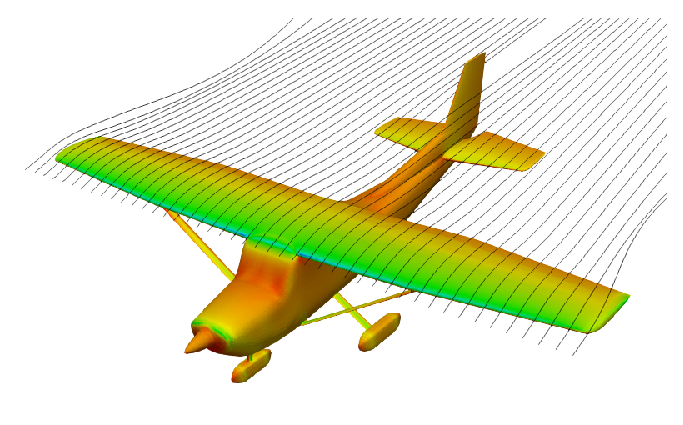
\includegraphics[width=110mm]{images/openfoam_results.eps}
  \caption{Streamlines and kinematic pressure distribution}
\end{figure}

If divergent or unstable behavior is observed decreasing under-relaxation factors defined in \texttt{relaxationFactors} dictionary in \texttt{system/fvSolution} file may improve solution convergence.
\begin{table}[h!]
  \begin{center}
    \begin{tabular}{ l | c }
      \toprule
      \textbf{Physical quantity} & \textbf{Under-Relaxation Factor} \\ \midrule
      Kinematic pressure          & 0.2 -- 0.3 \\
      Velocity                    & 0.5 -- 0.7 \\
      Turbulent kinetic energy    & 0.5 -- 0.7 \\
      Turbulence dissipation rate & 0.5 -- 0.7 \\
      \bottomrule
    \end{tabular}
    \caption{Commonly used under-relaxation factors \cite{FluentUserGuide15, Guerrero2018} }
  \end{center}
\end{table}

\section{Results}

\subsection{XFOIL}

XFOIL computations results, compared to the data available in \cite{NACA-TN-3361} and \cite{SheldahiKlimas1981}, are shown in figures \ref{fig-cfd-result-xfoil-cx}, \ref{fig-cfd-result-xfoil-cz} and \ref{fig-cfd-result-xfoil-cm}.

\subsection{VSPAERO}

VSPAERO computations results, compared to the OpenFOAM computations results, are shown in figures \ref{fig-cfd-result-vspaero-cx}, \ref{fig-cfd-result-vspaero-cz} and \ref{fig-cfd-result-vspaero-cm}.

\subsection{OpenFOAM}

OpenFOAM computations results, compared to the data available in \cite{NASA-TP-1538}, are shown in figures \ref{fig-cfd-result-openfoam-cx} and \ref{fig-cfd-result-openfoam-cz}.

\clearpage

\begin{figure}
  \centering
  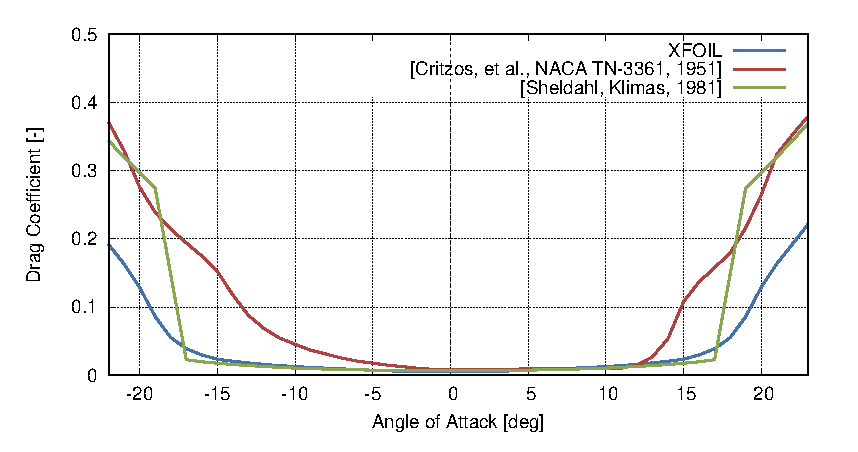
\includegraphics[width=140mm]{images/xfoil_naca0012_cx.eps}
  \caption{NACA 0012 drag coefficient}
  \label{fig-cfd-result-xfoil-cx}
\end{figure}

\begin{figure}
  \centering
  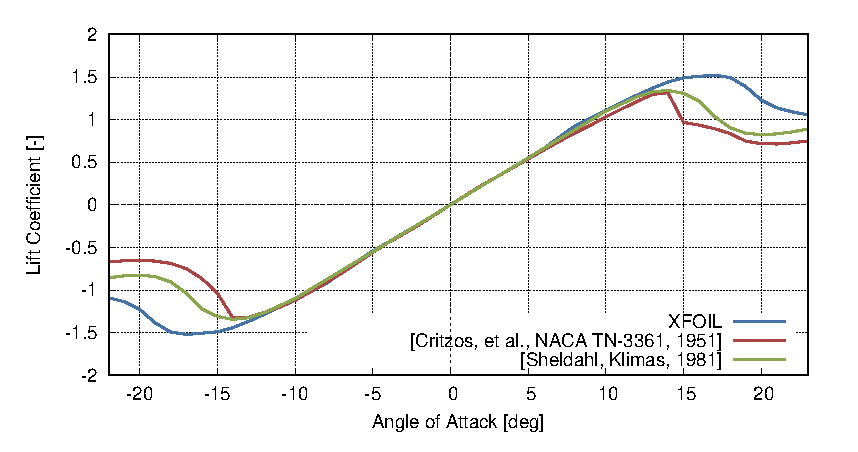
\includegraphics[width=140mm]{images/xfoil_naca0012_cz.eps}
  \caption{NACA 0012 lift coefficient}
  \label{fig-cfd-result-xfoil-cz}
\end{figure}

\begin{figure}
  \centering
  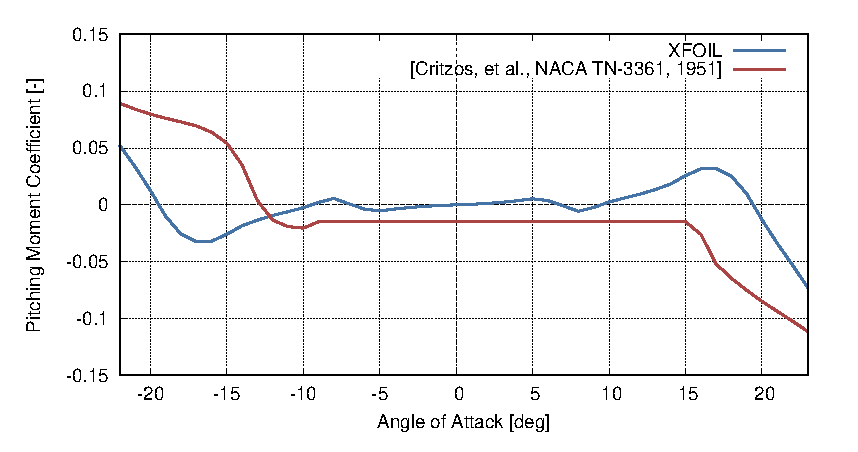
\includegraphics[width=140mm]{images/xfoil_naca0012_cm.eps}
  \caption{NACA 0012 pitching moment coefficient}
  \label{fig-cfd-result-xfoil-cm}
\end{figure}

\begin{figure}
  \centering
  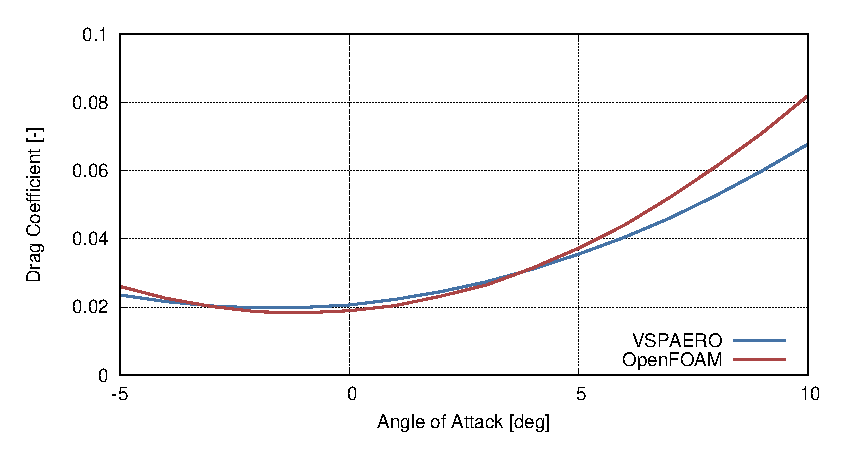
\includegraphics[width=140mm]{images/vspaero_p51_cx.eps}
  \caption{P-51 drag coefficient}
  \label{fig-cfd-result-vspaero-cx}
\end{figure}

\begin{figure}
  \centering
  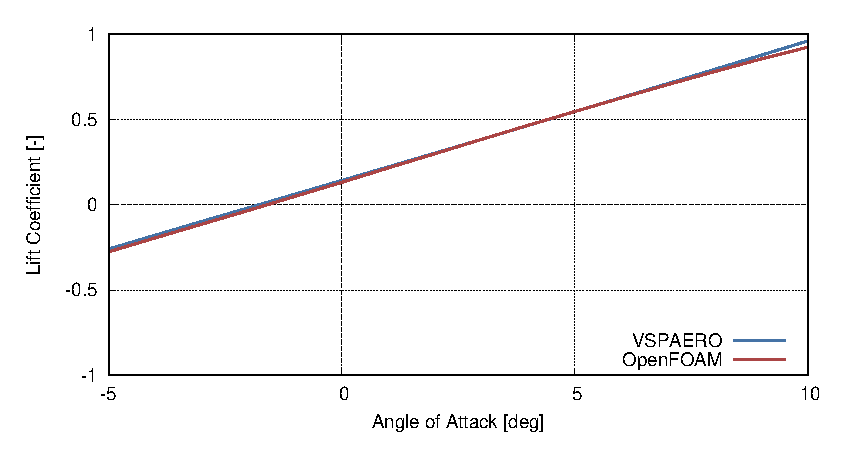
\includegraphics[width=140mm]{images/vspaero_p51_cz.eps}
  \caption{P-51 lift coefficient}
  \label{fig-cfd-result-vspaero-cz}
\end{figure}

\begin{figure}
  \centering
  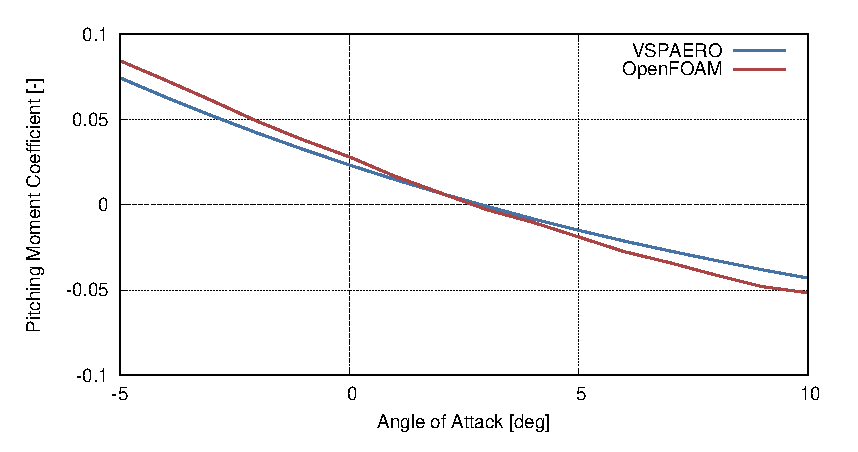
\includegraphics[width=140mm]{images/vspaero_p51_cm.eps}
  \caption{P-51 pitching moment coefficient}
  \label{fig-cfd-result-vspaero-cm}
\end{figure}

\begin{figure}
  \centering
  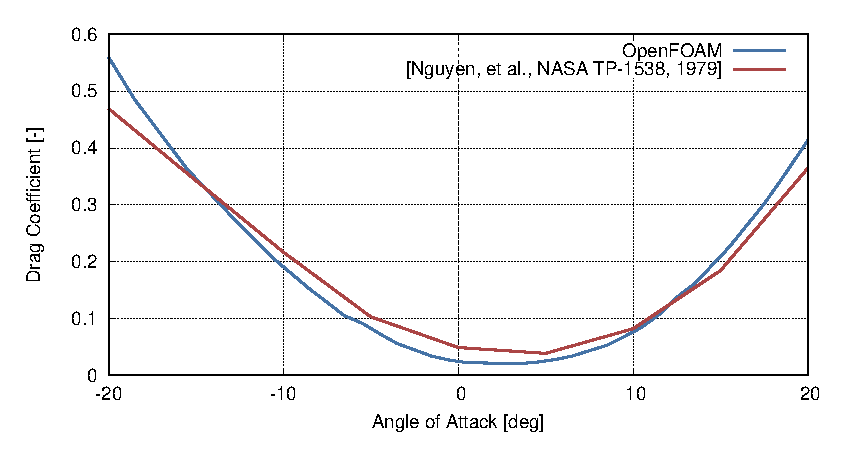
\includegraphics[width=140mm]{images/openfoam_f16_cx.eps}
  \caption{F-16 drag coefficient}
  \label{fig-cfd-result-openfoam-cx}
\end{figure}

\begin{figure}
  \centering
  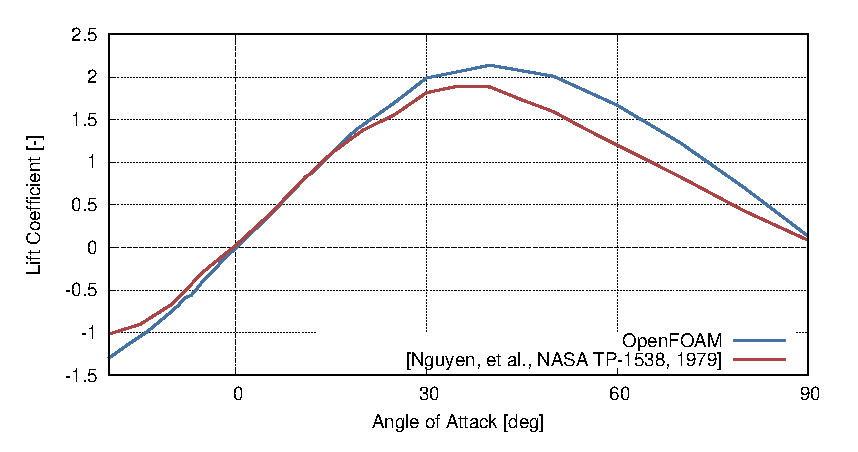
\includegraphics[width=140mm]{images/openfoam_f16_cz.eps}
  \caption{F-16 lift coefficient}
  \label{fig-cfd-result-openfoam-cz}
\end{figure}
